% =====================================================================
\section{The Gradient Vector}\label{ch:gradient}
% =====================================================================

\subsection{Definition}

The formula of Theorem~\ref{thm:Du-formula} has the shape of a dot product
(Slides, \emph{Gradient Vectors}):
\[
  \Du f(x,y)=f_x(x,y)\,a+f_y(x,y)\,b=\ip{f_x(x,y),\,f_y(x,y)}\cdot\ip{a,b}
  =\ip{f_x(x,y),\,f_y(x,y)}\cdot\vu .
\]
The first vector depends only on $f$ and the point, not on the direction. It
occurs so often that it gets a name.

\begin{definition}[Gradient; Slides]\label{def:grad}
If $f$ is a function of two variables $x$ and $y$, the \emph{gradient} of $f$
is the vector function $\grad f$ (read ``del $f$'', also written
$\operatorname{grad}f$) defined by
\[
  \grad f(x,y)=\ip{f_x(x,y),\,f_y(x,y)}=\pd{f}{x}\,\vi+\pd{f}{y}\,\vj .
\]
For a function of three variables,
$\grad f(x,y,z)=\ip{f_x,\,f_y,\,f_z}=\pd fx\vi+\pd fy\vj+\pd fz\vk$.
\end{definition}

\begin{keybox}{Directional derivative as a dot product}
If $f$ is differentiable and $\vu$ is a \emph{unit} vector, then
\[
  \Du f=\grad f\cdot\vu
\]
in two or three variables (Theorems~\ref{thm:Du-formula} and~\ref{thm:Du3}).
\end{keybox}

Note the types: $f$ is a scalar function, $\grad f$ is a \emph{vector}, and
$\Du f=\grad f\cdot\vu$ is again a \emph{scalar}. Writing $\grad f$ for a number
or $\Du f$ as a vector are common, costly mistakes.

\begin{example}[Slides, Example 6.3]\label{ex:6.3}
Find the gradient of $f(x,y)=y\ln x+xy^2$ at the point $(1,2)$.
\end{example}
\begin{solution}
\step{1}{Partial derivatives.} $f_x=\dfrac{y}{x}+y^2$ and $f_y=\ln x+2xy$.
\step{2}{Gradient.} $\grad f(x,y)=\ip{\dfrac yx+y^2,\;\ln x+2xy}$.
\step{3}{At $(1,2)$.}
\[
  \grad f(1,2)=\ip{\tfrac21+2^2,\;\ln1+2(1)(2)}=\ip{6,4}.
\]
\end{solution}

\begin{example}[Slides, Example 6.4 via the gradient]
Redo Example~\ref{ex:6.4} using $\Du f=\grad f\cdot\vu$.
\end{example}
\begin{solution}
$\grad f(x,y)=\ip{6x,-4y}$, so $\grad f\left(-\tfrac34,0\right)=\ip{-\tfrac92,0}$; with
$\vu=\ip{\tfrac35,\tfrac45}$,
\[
  \Du f\left(-\tfrac34,0\right)=\ip{-\tfrac92,0}\cdot\ip{\tfrac35,\tfrac45}=-\frac{27}{10}.
\]
\emph{Caution:} the slide prints the middle step as $\ip{-9,0}$, but
$6\left(-\frac34\right)=-\frac92$, not $-9$. With $\ip{-9,0}$ one would get
$-\frac{27}{5}$; the slide's final answer $-\frac{27}{10}$ is the correct one,
coming from $\ip{-\frac92,0}$.
\end{solution}

\subsection{Maximizing the directional derivative}

Let $\theta$ be the angle between $\grad f$ and the unit vector $\vu$. By the
geometric form of the dot product (Slides),
\[
  \Du f=\grad f\cdot\vu=\norm{\grad f}\,\norm{\vu}\cos\theta=\norm{\grad f}\cos\theta,
\]
because $\norm{\vu}=1$. Everything about the size of $\Du f$ is now controlled
by the single number $\cos\theta\in[-1,1]$ (Figure~\ref{fig:angle}).

\begin{figure}[H]
\centering
\begin{tikzpicture}[scale=1.6,>=Stealth]
  \draw[->,very thick,BrickRed] (0,0) -- (2.4,1.2) node[right]{$\grad f(x_0,y_0)$};
  \draw[->,very thick,NavyBlue] (0,0) -- (0.6,1.3) node[above]{$\vu$ \ (unit)};
  \draw[dashed] (0.6,1.3) -- (1.0,0.5);
  \draw[line width=2.2pt,ForestGreen] (0,0) -- (1.0,0.5);
  \node[ForestGreen,below right] at (0.45,0.15) {$\cos\theta$};
  \draw ({0.45*cos(26.57)},{0.45*sin(26.57)}) arc[start angle=26.57,end angle=65.22,radius=0.45];
  \node at ({0.62*cos(46)},{0.62*sin(46)}) {$\theta$};
  \fill (0,0) circle (1pt) node[below left]{$(x_0,y_0)$};
\end{tikzpicture}
\caption{$\Du f=\norm{\grad f}\cos\theta$. The green segment is the projection
of the unit vector $\vu$ onto the direction of $\grad f$; it has signed length
$\cos\theta$. It is longest when $\vu$ points along $\grad f$.}
\label{fig:angle}
\end{figure}

\begin{theorem}[Maximum rate of change; Slides]\label{thm:max}
Let $f$ be differentiable at $P$ with $\grad f(P)\neq\vzero$. Then, as $\vu$
ranges over all unit vectors:
\begin{enumerate}[label=(\alph*)]
  \item the \textbf{maximum} value of $\Du f(P)$ is $\norm{\grad f(P)}$, attained
        exactly when $\vu$ points in the direction of $\grad f(P)$, i.e.
        $\vu=\grad f(P)/\norm{\grad f(P)}$ ($\theta=0$);
  \item the \textbf{minimum} value is $-\norm{\grad f(P)}$, attained when $\vu$
        points in the direction of $-\grad f(P)$ ($\theta=\pi$);
  \item $\Du f(P)=0$ exactly when $\vu\perp\grad f(P)$ ($\theta=\frac\pi2$);
  \item every value in $\left[-\norm{\grad f(P)},\;\norm{\grad f(P)}\right]$ is
        attained, and no other value is.
\end{enumerate}
If $\grad f(P)=\vzero$, then $\Du f(P)=0$ for every $\vu$.
\end{theorem}

\begin{proof}
Since $-1\le\cos\theta\le1$, we get
$-\norm{\grad f}\le\norm{\grad f}\cos\theta\le\norm{\grad f}$. The value
$\cos\theta=1$ occurs only for $\theta=0$, i.e. $\vu$ has the direction of
$\grad f$; $\cos\theta=-1$ only for $\theta=\pi$; $\cos\theta=0$ only for
$\theta=\frac\pi2$. As $\theta$ varies continuously from $0$ to $\pi$,
$\cos\theta$ takes every value in $[-1,1]$, giving (d).
\end{proof}

\begin{keybox}{In words}
The gradient $\grad f$ points in the direction in which $f$ \emph{increases
most rapidly}, and its length $\norm{\grad f}$ is that maximum rate of
increase. $-\grad f$ is the direction of fastest decrease. Directions
perpendicular to $\grad f$ are directions of no instantaneous change.
\end{keybox}

\begin{example}\label{ex:xey}
Let $f(x,y)=xe^y$.
(a) Find the rate of change of $f$ at $P(2,0)$ in the direction from $P$ to
$Q\left(\tfrac12,2\right)$.
(b) In what direction does $f$ have the maximum rate of change at $P$? What is
this maximum rate?
\end{example}
\begin{solution}
\step{1}{Gradient.} $\grad f(x,y)=\ip{e^y,\;xe^y}$, so $\grad f(2,0)=\ip{1,2}$.

\textbf{(a)} $\vecPQ=\ip{\tfrac12-2,\;2-0}=\ip{-\tfrac32,2}$. Scale by $2$:
$\ip{-3,4}$ has the same direction and length $5$, so $\vu=\ip{-\tfrac35,\tfrac45}$.
\[
  \Du f(2,0)=\ip{1,2}\cdot\ip{-\tfrac35,\tfrac45}=-\tfrac35+\tfrac85=1 .
\]

\textbf{(b)} By Theorem~\ref{thm:max}, $f$ increases fastest in the direction of
$\grad f(2,0)=\ip{1,2}$ (unit vector $\ip{\tfrac{1}{\sqrt5},\tfrac{2}{\sqrt5}}$),
and the maximum rate is $\norm{\ip{1,2}}=\sqrt5\approx2.24$.

Figure~\ref{fig:du-theta} plots $\Du f(2,0)=\cos\theta+2\sin\theta$ against the
angle $\theta$ of $\vu$: it oscillates between $-\sqrt5$ and $\sqrt5$, exactly
as Theorem~\ref{thm:max} predicts.
\end{solution}

\begin{figure}[H]
  \centering
  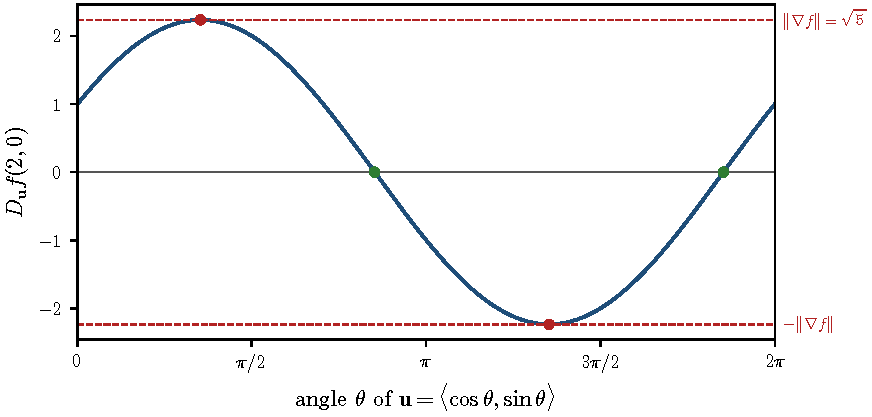
\includegraphics[width=0.78\linewidth]{du_vs_theta}
  \caption{$\Du f(2,0)$ for $f=xe^y$ as $\vu$ turns once around the circle. Red:
  maximum $\sqrt5$ at $\theta=\arctan2$ (the direction of $\grad f$) and minimum
  $-\sqrt5$ half a turn later. Green: the two directions perpendicular to
  $\grad f$, where the rate is $0$.}
  \label{fig:du-theta}
\end{figure}

\subsection{The trio activity, solved}

\begin{example}[Slides, Activity (by trio)]\label{ex:trio}
Let $f(x,y)=200e^{-x^2-3y^2}$.
\begin{enumerate}[label=(\alph*)]
  \item Find the directional derivative of $f$ at $P(4,-1)$ in the direction toward $Q(7,3)$.
  \item Determine the direction in which $f$ increases most rapidly at $P$.
  \item Find the maximum rate of increase of $f$ at $P$.
\end{enumerate}
\end{example}
\begin{solution}
\step{1}{Gradient.} By the chain rule,
\[
  f_x=200e^{-x^2-3y^2}\cdot(-2x)=-400x\,e^{-x^2-3y^2},\qquad
  f_y=200e^{-x^2-3y^2}\cdot(-6y)=-1200y\,e^{-x^2-3y^2}.
\]
These are continuous, so $f$ is differentiable.
\step{2}{At $P(4,-1)$.} The exponent is $-16-3=-19$, so
\[
  \grad f(4,-1)=\ip{-1600e^{-19},\;1200e^{-19}}=400e^{-19}\ip{-4,3}.
\]
\textbf{(a)} $\vecPQ=\ip{7-4,\;3-(-1)}=\ip{3,4}$, $\norm{\vecPQ}=5$,
$\vu=\ip{\tfrac35,\tfrac45}$. Hence
\[
  \Du f(4,-1)=400e^{-19}\ip{-4,3}\cdot\ip{\tfrac35,\tfrac45}
  =400e^{-19}\left(-\tfrac{12}{5}+\tfrac{12}{5}\right)=0 .
\]
\textbf{(b)} The direction of $\grad f(4,-1)$, i.e. of $\ip{-4,3}$; as a unit
vector, $\ip{-\tfrac45,\tfrac35}$.

\textbf{(c)} $\norm{\grad f(4,-1)}=400e^{-19}\sqrt{16+9}=2000e^{-19}\approx1.12\times10^{-5}$.

\textbf{Why is (a) zero?} The level curves of $f$ are the ellipses
$x^2+3y^2=c$. The one through $P$ is $x^2+3y^2=19$, and the direction
$\ip{3,4}$ is tangent to it at $P$ (it is perpendicular to $\grad f(P)\parallel\ip{-4,3}$).
Moving along a level curve, $f$ does not change to first order, so the rate is
$0$ (Theorem~\ref{thm:max}(c); Figure~\ref{fig:trio}).
\end{solution}

\begin{figure}[H]
  \centering
  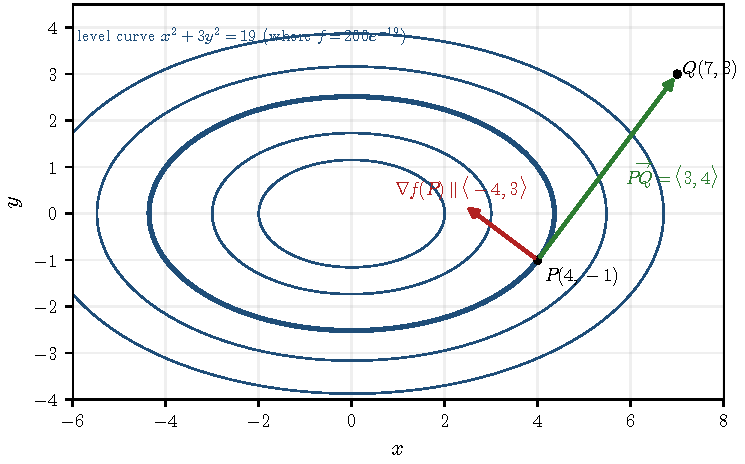
\includegraphics[width=0.72\linewidth]{trio_activity}
  \caption{Trio activity. $\protect\vecPQ$ (green) is tangent to the level
  curve through $P$, so it is perpendicular to the gradient (red) and the
  directional derivative is $0$.}
  \label{fig:trio}
\end{figure}

\subsection{More examples}

\begin{example}[Three variables]\label{ex:temp3}
The temperature at $(x,y,z)$ is $T(x,y,z)=\dfrac{80}{1+x^2+2y^2+3z^2}$
($^\circ$C, metres). In which direction does the temperature increase fastest at
$(1,1,-2)$? What is the maximum rate of increase?
\end{example}
\begin{solution}
\step{1}{Gradient.} Write $T=80\,D^{-1}$ with $D=1+x^2+2y^2+3z^2$. Then
$T_x=-80D^{-2}\cdot2x$, etc.:
\[
  \grad T=\frac{-80}{(1+x^2+2y^2+3z^2)^2}\ip{2x,\;4y,\;6z}.
\]
\step{2}{At $(1,1,-2)$.} $D=1+1+2+12=16$, so
\[
  \grad T(1,1,-2)=\frac{-80}{256}\ip{2,4,-12}=\frac{-5}{16}\ip{2,4,-12}=\frac58\ip{-1,-2,6}.
\]
\step{3}{Answer.} The temperature increases fastest in the direction of
$\ip{-1,-2,6}$ (unit vector $\frac{1}{\sqrt{41}}\ip{-1,-2,6}$); the maximum rate is
\[
  \norm{\grad T(1,1,-2)}=\frac58\sqrt{1+4+36}=\frac{5\sqrt{41}}{8}\approx4.00\ ^\circ\text{C/m}.
\]
\end{solution}

\begin{example}[Finding directions with a prescribed rate]\label{ex:prescribed}
Let $f(x,y)=x^2y$ and $P(1,2)$.
(a) Find all unit vectors $\vu$ with $\Du f(P)=1$.
(b) Find all $\vu$ with $\Du f(P)=0$.
(c) Is there a direction with $\Du f(P)=5$?
\end{example}
\begin{solution}
\step{1}{Gradient.} $\grad f=\ip{2xy,\,x^2}$, so $\grad f(1,2)=\ip{4,1}$ and
$\norm{\grad f(1,2)}=\sqrt{17}\approx4.12$.

\textbf{(a)} Let $\vu=\ip{a,b}$. We need
\[
  4a+b=1\qquad\text{and}\qquad a^2+b^2=1 .
\]
From the first, $b=1-4a$. Substituting: $a^2+(1-4a)^2=1\iff17a^2-8a=0\iff a(17a-8)=0$.
\begin{itemize}
  \item $a=0\Rightarrow b=1$: $\vu=\ip{0,1}$.
  \item $a=\frac{8}{17}\Rightarrow b=1-\frac{32}{17}=-\frac{15}{17}$: $\vu=\ip{\frac{8}{17},-\frac{15}{17}}$.
\end{itemize}
Check: $4(0)+1=1$\checkok; $\frac{32}{17}-\frac{15}{17}=1$\checkok. Two directions,
symmetric about $\grad f$, as expected from $\Du f=\sqrt{17}\cos\theta$, where
$\cos\theta=1/\sqrt{17}$ has two solutions $\pm\theta$.

\textbf{(b)} $\vu\perp\ip{4,1}$: $\vu=\pm\frac{1}{\sqrt{17}}\ip{1,-4}$.

\textbf{(c)} No: $5>\sqrt{17}=\norm{\grad f(P)}$, the largest possible value
(Theorem~\ref{thm:max}(d)).
\end{solution}

\subsection{Rules for gradients}

Because partial derivatives obey the usual rules, so does $\grad$. For
differentiable $f,g$ and constants $\alpha,\beta$:
\[
  \grad(\alpha f+\beta g)=\alpha\grad f+\beta\grad g,\qquad
  \grad(fg)=f\grad g+g\grad f,\qquad
  \grad\!\left(\frac fg\right)=\frac{g\grad f-f\grad g}{g^2},
\]
and for a differentiable one-variable function $F$, the chain rule gives
$\grad\big(F(f)\big)=F'(f)\,\grad f$.

\begin{example}[Gradient of distance]\label{ex:grad-r}
Let $r=\sqrt{x^2+y^2+z^2}$ be the distance from the origin and
$\vx=\ip{x,y,z}$. Show that $\grad r=\dfrac{\vx}{r}$ and
$\grad\!\left(\dfrac1r\right)=-\dfrac{\vx}{r^3}$ for $\vx\neq\vzero$.
\end{example}
\begin{solution}
\step{1}{$\grad r$.} $\pd rx=\dfrac{1}{2\sqrt{x^2+y^2+z^2}}\cdot2x=\dfrac xr$, and
likewise $\pd ry=\dfrac yr$, $\pd rz=\dfrac zr$. So $\grad r=\dfrac1r\ip{x,y,z}=\dfrac{\vx}{r}$:
a unit vector pointing directly away from the origin (distance grows fastest
moving radially outward, at rate $1$).
\step{2}{$\grad(1/r)$.} With $F(s)=1/s$, $F'(s)=-1/s^2$, the chain rule gives
\[
  \grad\!\left(\frac1r\right)=-\frac1{r^2}\,\grad r=-\frac{1}{r^2}\cdot\frac{\vx}{r}=-\frac{\vx}{r^3}.
\]
This vector field, pointing toward the origin with magnitude $1/r^2$, is the
shape of Newton's gravitational field; it reappears in Lecture Notes No.~7.
\end{solution}

\begin{remark}[Looking ahead]
$\grad f$ assigns a vector to every point of the domain, so it is a
\emph{vector field}: the \emph{gradient field} of $f$. Vector fields, gradient
fields and their ``potential functions'' are the topic of Lecture Notes
No.~7 (Slides~7, \emph{Vector Calculus}).
\end{remark}
